\documentclass[a4paper]{article}

\usepackage{fullpage} % Package to use full page
\usepackage{parskip} % Package to tweak paragraph skipping
\usepackage{tikz} % Package for drawing
\usepackage{amsmath}
\usepackage{float}
\usepackage{hyperref}
\usepackage{amssymb}
\usepackage[nodisplayskipstretch]{setspace}
\setstretch{0.5}
\usepackage{listings}
\usepackage{color}
 
\definecolor{codegreen}{rgb}{0,0.6,0}
\definecolor{codegray}{rgb}{0.5,0.5,0.5}
\definecolor{codepurple}{rgb}{0.58,0,0.82}
\definecolor{backcolour}{rgb}{0.95,0.95,0.92}
 
\lstdefinestyle{mystyle}{
    backgroundcolor=\color{backcolour},   
    commentstyle=\color{codegreen},
    keywordstyle=\color{magenta},
    numberstyle=\tiny\color{codegray},
    stringstyle=\color{codepurple},
    basicstyle=\footnotesize,
    breakatwhitespace=false,         
    breaklines=true,                 
    captionpos=b,                    
    keepspaces=true,                 
    numbers=left,                    
    numbersep=5pt,                  
    showspaces=false,                
    showstringspaces=false,
    showtabs=false,                  
    tabsize=2
}

\title{MAST30013 - Techniques in Operations Research: Assignment 1}
\author{Shreyash Patodia (767336)}
\date{19/03/2018}

\begin{document}

\maketitle

\section*{Question 1}

\subsection*{1(a):}

Below is a plot of $f(x) = 8e^{1 -x} + 7log(x)$ in the interval $[1, 2]$:
\begin{figure}[!htbp]
\begin{center}
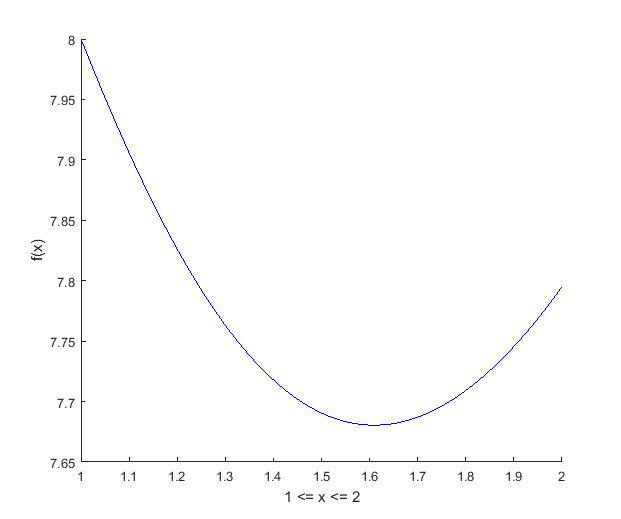
\includegraphics[scale=0.75]{problem-1.png}
\end{center}
\caption{Plot of $f(x) = 8e^{1 -x} + 7log(x)$ in the interval $[1, 2]$:}\label{exampleplot}
\end{figure}

The above plot clearly shows that $f(x)$ is unimodal since it only has one local minima.

\subsection*{1(b):}

In order to perform Fibonacci Search we first need to find the smallest $n$ such that $F_n(\alpha) = (b - a)$. Thus, we need to find an $n$ where $\alpha  < 2\epsilon$ or we need:
\begin{equation}
(b - a)/F_n < 2\epsilon
\end{equation}
\begin{equation}
F_n > (b - a)/2\epsilon
\end{equation}
Setting $b = 2, a = 1$ and $\epsilon = 0.08$ we get:
\begin{equation}
F_n > \dfrac{2 - 1}{2 * 0.08}
\end{equation}
\begin{equation}
F_n > \dfrac{1}{0.16}
\end{equation}
\begin{equation}
F_n > 6.25
\end{equation}

So, $F_n = 8$ and $n = 5$.

Now, we know $f(x)$, we know the interval is $[1, 2]$ and the initial $k = 5$.  We will also use the following formulas for p and q:

\begin{equation}
a = 1
\end{equation}

\begin{equation}
b = 2
\end{equation}

\begin{equation}
p = b - \dfrac{F_{k - 1}}{F{k}}(b - a)
\end{equation}

\begin{equation}
q = a + \dfrac{F_{k - 1}}{F{k}}(b - a)
\end{equation}

After, that we will use $f(p)$ and $f(q)$ to evaluate how to reduce the intervals.

%%%%%%%%%%%%%%%%%%%%%%%
\begin{equation}
k = n = 5
\end{equation}

\begin{equation}
p = 2 - \dfrac{5}{8} * (1) = 2 - \dfrac{5}{8} = 1.375
\end{equation}

\begin{equation}
q = 1 + \dfrac{5}{8} * (1)  = 1 + \dfrac{5}{8} = 1.625
\end{equation}

\begin{equation}
f(p) = 7.7275
\end{equation}   

\begin{equation}
f(q) = 7.6806
\end{equation}

Now, since $f(p) > f(q)$ the new interval will have:

\begin{equation}
a = p = 1.375
\end{equation}

\begin{equation}
b = 2
\end{equation}

\begin{equation}
p = q = 1.625
\end{equation}

%%%%%%%%%%%%%%%%%%%%%%%%%%%%%%%%%%%%


%%%%%%%%%%%%%%%%%%%%%%%
\begin{equation}
k = n = 4
\end{equation}

\begin{equation}
q = 1.375 + \dfrac{3}{5} * (0.625)  = 1.75
\end{equation}

\begin{equation}
f(p) = 7.6806    
\end{equation}   

\begin{equation}
f(q) = 7.6962
\end{equation}

Now, since $f(q) > f(p)$ the new interval will have:

\begin{equation}
a = 1.375
\end{equation}
\begin{equation}
b = q = 1.75
\end{equation}

\begin{equation}
q  = p = 1.625
\end{equation}

%%%%%%%%%%%%%%%%%%%%%%%%%%%%%%%%%%%%

%%%%%%%%%%%%%%%%%%%%%%%
\begin{equation}
k = n = 3
\end{equation}

\begin{equation}
p = 1.75 -  \dfrac{2}{3} * (0.375)  = 1.5
\end{equation}

\begin{equation}
f(p) = 7.6905   
\end{equation}   

\begin{equation}
f(q) =  7.6806
\end{equation}

Now, since $f(p) > f(q)$ the new interval will have:

\begin{equation}
a = p = 1.5
\end{equation}
\begin{equation}
b = 1.75
\end{equation}

\begin{equation}
p  = q = 1.625
\end{equation}

%%%%%%%%%%%%%%%%%%%%%%%%%%%%%%%%%%%%

\begin{equation}
k = 2
\end{equation}

Because $k = 2$ we will have to set q as below:

\begin{equation}
q = a + 2\epsilon = 1.660
\end{equation}

\begin{equation}
f(p) = 7.6806    
\end{equation}

\begin{equation}
f(q) = 7.6825
\end{equation}

Now, since $f(p) < f(q)$ the new interval will have:

\begin{equation}
a = 1.5
\end{equation}
\begin{equation}
b = q = 1.660
\end{equation}

Thus, the final interval found using fibonacci search is $[1.5, 1.66]$ which is withing the tolerance required. 

Thus $x^* = 1.58 \pm 0.08$.

\section*{Question 2}

Let us first try to find a $b$ such that $[0, b]$ contains the minimum. But first we need to check that $f(x)$ is unimodal.
Given:
\begin{equation}
f(x) = (40x+1) log(40x+1)−200x
\end{equation}

Plotting $f(x)$ in the interval $[0, 12]$ we get 

\begin{figure}[H]
\begin{center}
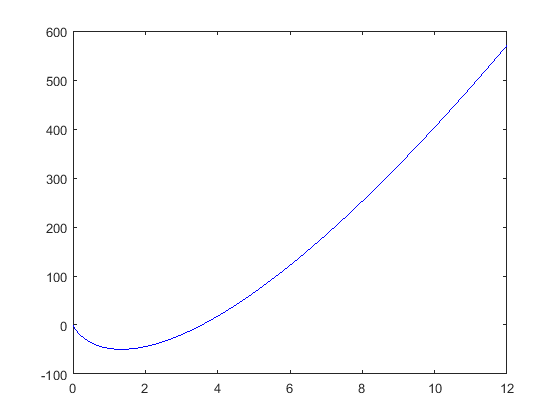
\includegraphics[scale=0.75]{problem-2.png}
\end{center}
\caption{Plot of $f(x) = (40x+1) log(40x+1) - 200x$ in the interval $[0, 12]$:}\label{exampleplot}
\end{figure}

Also, let $f'$ is:
\begin{equation}
f'(x) = 40log(40x + 1) - 160
\end{equation}

Setting $f'(x) = 0$:
\begin{eqnarray}
f'(x) &=& 0 \\
40log(40x + 1) - 160 &=& 0 \\
log(40x + 1) - 4 &=& 0 \\
log(40x + 1) &=& 4 \\ 
x &=& \dfrac{e^4 - 1}{40} \\ 
\end{eqnarray}

This shows there is one value for which $f'(x) = 0$ and from the graph we can see this value to be between 0 and 5. Thus, the given function is unimodal and continuous (from the graph and because there are no points where the function wouldn't be defined in $[0, \infty]$ allowing us to use Golden Section Search. 

Let us try to find a good interval to do our search in. Assuming T (a small increment):
$T = 1$

Set $k = 1$:
\begin{equation}
p = 0
\end{equation}
\begin{equation}
q = T
\end{equation}

\begin{equation}
f(p) = f(0) =  0
\end{equation}
\begin{equation}
f(q) = f(1) = -47.7435
\end{equation}

So, $f(p) > f(q)$. Set $k = 2$ :

\begin{equation}
p = q = 1
\end{equation}
\begin{equation}
q = p + 2^{k - 1}T = 1 + 2*1 = 3
\end{equation}

\begin{equation}
f(p) = f(1) = -47.7435
\end{equation}

\begin{equation}
f(q) = -19.7093
\end{equation}


Thus, $ f(p) < f(q)$, meaning the minimum lies in the range: $[0, 3]$.  As $f(p) > f(q)$ for $k = 1$  and $f(p) < f(q)$ for $k = 2$.

We can now perform the Golden Section Search in the interval $[0, 3]$. Now, let us determine the number of calculations needed ($a = 0$, $b = 3$, $\epsilon = 0.3$):

\begin{equation}
a = 0
\end{equation}
\begin{equation}
b = 3
\end{equation}

\begin{eqnarray}
\gamma^n (b - a) &<& 2\epsilon\\ 
0.6180^n &<& \dfrac{0.6}{3}\\
0.6180^n &<& 0.2 \\
0.6180^4 = 0.1459 &<& 0.2
\end{eqnarray}

Thus, $ n = 4 $ which means we need to do 5 f calculations.

\begin{equation}
p = b - \gamma(b - a) = 3 - 0.6180(3) = 1.146
\end{equation}
\begin{equation}
q = a + \gamma(b - a) = 0 + 0.6180(3) = 1.854
\end{equation}
\begin{equation}
f(p) = -49.0182
\end{equation}
\begin{equation}
f(q) = -46.1361
\end{equation}

Since, $f(q) > f(p)$, we can set the new $b = q = 1.854$ and $a = 0$ remains the same. We have $3$ f calculations left (Also, $q = p = 1.146$):

\begin{equation}
p = 1.854  - 0.6180*(1.854) = 0.7082
\end{equation}
\begin{equation}
f(p) = -42.5542
\end{equation}

\begin{equation}
f(q) = -49.0182
\end{equation}

Since, $f(p) > f(q)$. We get $a = p = 0.7082 $, $p = q = 1.146$ and $b = 1.854$ remains the same. We now have just $2$ f calculations left. 

Now, 

\begin{equation}
q = 0.7082 + 0.6180*(1.1458) = 1.4163
\end{equation}
\begin{equation}
f(p) = -49.0182
\end{equation}

\begin{equation}
f(q) = -49.5141
\end{equation}

Since, $f(p) > f(q)$, we make $a = p = 1.146$, $p = q = 1.4163$ and $b = 1.854$ remains the same. Doing the last f calculation. 

\begin{equation}
q = 1.146 + 0.6180*(0.708) = 1.5834
\end{equation}
\begin{equation}
f(p) = -49.5141
\end{equation}
\begin{equation}
f(q) = -48.7760
\end{equation}

Finally, since $f(q) > f(p)$ then the final $a = 1.146$ and the final $b = q = 1.5834$. Thus, the interval for minimisation is $[1.146, 1.583]$.  Which means $x^* = 1.3645 \pm 0.2185$.

\section*{Question 3}

Given:

$
f(x) = (2x − 1)^3 + 4(4 − 10x)^4
$

We can find $f'(x)$ to be as follows:

$f'(x) = 6(2x - 1)^2  - 1280(2 - 5x)^3$ 

The above functions $f$ and  $f'$ are a combination of two polynomials and polynomials are continuous for all real numbers, so the functions are continuous for all real numbers.

First we need to find a t that satisfies the Armijo-Goldstein condition and the Wolfe condition so that we can find an interval where the solution might lie in. Since, $\sigma \in [0, 1]$ we can assume it to be $0.5$, similarly $\mu \in [\sigma, 1)$ so we can let $\sigma = 0.75$.  Set $t_{lo} = 0$ and $t_{hi} = \infty$ and $t = 1$

\begin{equation}
f(0) = 1023
\end{equation}

\begin{equation}
f(t) = f(1) =  5185
\end{equation}

\begin{equation}
f(t) > f(0) + t{\sigma}f'(0) = -4094
\end{equation}

So, $t_{hi} = 1$, $t = \dfrac{1}{2}(t_{lo} + t_{hi}) = \dfrac{1}{2}$. Now, 

\begin{equation}
f(t) = f(0.5) = 4
\end{equation}

\begin{equation}
f(0) + t{\sigma}f'(0) = −1536
\end{equation}

\begin{equation}
\therefore f(t) > f(0) + t{\sigma}f'(0)
\end{equation}

So, $t_{hi} = 0.5$, $t = \dfrac{1}{2}(t_{lo} + t_{hi}) = \dfrac{1}{4}$. Now, 

\begin{equation}
f(t) = f(0.25) = 20.1250
\end{equation}

\begin{equation}
f(0) + t{\sigma}f'(0) = −256.25
\end{equation}

\begin{equation}
\therefore f(t) > f(0) + t{\sigma}f'(0)
\end{equation}

So, $t_{hi} = 0.25$, $t = \dfrac{1}{2}(t_{lo} + t_{hi}) = \dfrac{1}{8}$. Now, 

\begin{equation}
f(t) = f(0.125) = 228.3438
\end{equation}

\begin{equation}
f(0) + t{\sigma}f'(0) = 383
\end{equation}

\begin{equation}
\therefore f(t) < f(0) + t{\sigma}f'(0)
\end{equation}

\begin{equation}
f'(t) = f'(0.125) = -3324
\end{equation}

\begin{equation}
{\mu}f'(0) = -7676
\end{equation}

\begin{equation}
\therefore f'(t) > {\mu}f'(0)
\end{equation}

Since, $f'(t) > {\mu}f'(0)$  we can stop and choose the step size to be $t = 0.125$. 

Also, $f'(x) = 6(2x - 1)^2  - 1280(2 - 5x)^3$  has only one real root so the function has to be unimodal from the graph below:

\begin{figure}[!htbp]
\begin{center}
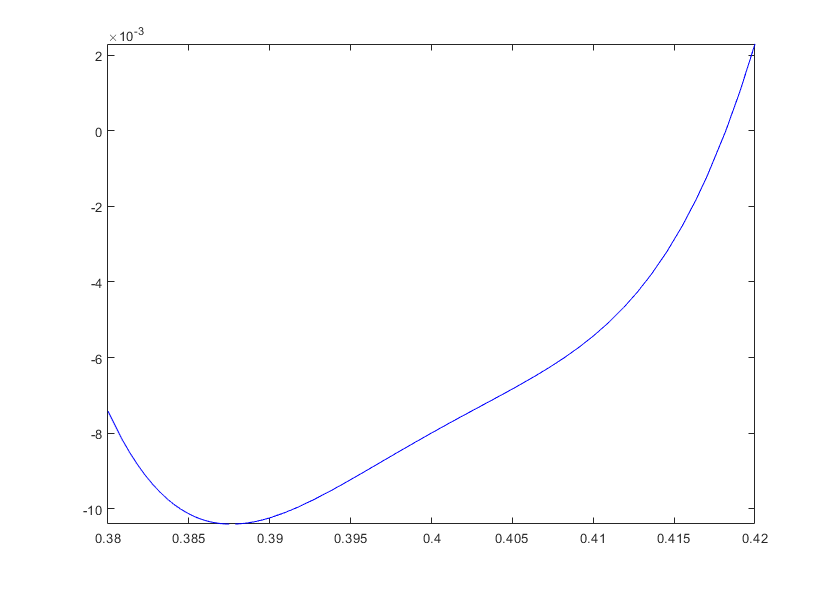
\includegraphics[scale=0.75]{problem-3.png}
\end{center}
\caption{Plot of $f(x) = 8e^{1 -x} + 7log(x)$ in the interval $[1, 2]$:}\label{exampleplot}
\end{figure}

Now, we want to use this step size to find an interval in which we can apply the Method of False Position. Now, because the interval in unbounded, we need to bound it in at least one direction first. Let us set $a = 0$ and with $t = 0.125$ we get: 

\begin{equation}
f(a) = f(0) = 1023
\end{equation}
\begin{equation}
f(a + T) = f(0.125) = 228.3438
\end{equation}

Since, $f(a) > f(a + T)$ we can close the interval on the left and use $[0, \infty)$ as our starting point. 

Now, finally we need to find an interval to apply Method of False Position by finding a suitable interval. I will use the method of increasing by a factor of t each time since a lot of the relevant calculations have been done above and wouldn't need to be done again. Here we start from 0 and $t = 0.125$

\begin{equation}
f(0) = 1023
\end{equation}

\begin{equation}
f(t) = f(0.125) = 228.3438
\end{equation}

\begin{equation}
f(2t) = f(0.25) = 20.1250
\end{equation}

\begin{equation}
f(3t) = f(0.375) = 0
\end{equation}

\begin{equation}
f(4t) = f(0.500) = 4
\end{equation}

Since we know that $2t = 0.25$ is in the decreasing branch and $4t = 0.5$ is in the increasing branch we can use this as our interval to find the answer. So interval = $[0.25, 0.50]$.

We can put this in our code to find the answer: 

\begin{lstlisting}[language=Octave]

function val = F(x)
val = (2 * x - 1)^3 + 4 * (4 - 10 * x)^4

function val = Fprime(x)
val = 6 * (2 * x - 1)^2 - 1280 * (2 - 5 * x)^3

function [root, val, iterations] = FalsePosition(fprime, a, b, epsilon)
format long g
k = 1
ga = feval(fprime, a)
gb = feval(fprime, b)
p = a + ((b - a) * ga)/(ga - gb)
gp = feval(fprime, p)

while abs(gp) > epsilon
    if gp < 0
        a = p
    else
        b = p
    end
    p = a + ((b - a) * ga)/(ga - gb)
    gp = feval(fprime, p)
    k = k + 1
end

root = p
val = gp
iterations = k

\end{lstlisting}

The above code gives the solution:

\begin{equation}
root = 0.387627049693125
\end{equation}


\begin{equation}
val = -3.47558047975038e-06
\end{equation}

\begin{equation}
iterations = 25
\end{equation}

The value observed above is within the tolerance. 

\end{document}